\section{Experimental evaluation}
\label{sec_exp}

Now we describe the results of applying our shield synthesis method to several examples. We use the reactive synthesis tool \texttt{Slugs}~\cite{EhlersR16} to compute locally-optimal shields
under the assumption, that sequences of wrong outputs are bounded by a constant $b$, as discussed in Section~\ref{sec:shieldsynth-local}.
All experiments were  performed on an Intel i5-5300U 2.30 GHz CPU with 8 GB of RAM.

\subsection{Gridworld}\label{exp:gridworld}
In the first set of experiments, we consider a gridworld with two agents that can move in one of the four cardinal directions at each time step. One grid cell is designated as a charging station. We require global safety property $\spec = \spec_{collision} \wedge \spec_{charge}$, where $\spec_{collision}$ requires collision avoidance and no simultaneous charging, and $\spec_{charge}$ describes when and how the agents should use the charging station.
  The formula $\spec_{charge}$ is of the form $\spec_{charge,1} \wedge \spec_{charge,2}$. These properties are specified in LTL as follows:
  \vspace{-0.3cm}

  \begin{align}\label{eqn:safety2}
  \spec_{charge,i} &= &\LTLglobally\Big(charging_i \rightarrow \lnot \LTLnext charging_j				\Big) \nonumber \\
  \spec_{collision} &=&\LTLglobally \lnot \Big(position_i = position_j				\Big)
  \end{align}
  for $i,j \in \{1,2\}$ and $i \neq j$. The formula $\spec_{charge,i}$ requires that one agent cannot enter the charging area right  after the other one has left. The integer variable $position_i$ is the position of agent $i$ in the grid. $\spec_{collision}$ requires that the agents do not occupy the same position.

We synthesized locally-optimal shields using an interference cost function $c$ that assigns higher costs for any interferences with
the first agent than for interferences with the second one. We consider different values for the bound $b$ on the length of sequences of wrong outputs. A larger bound $b$ results in more robust shields, but also in larger state-spaces of the game, due to the size of the counter that augments the state space.

We report the results in Table~\ref{tab:exp1shield} under case (1).
The first column gives the bound $b$, the second and the third column state the number of input and output bits of $\varphi$.
The fourth column states the total number of variables of the constructed game (including the variables that augment the state space)
and the fifth column gives the number of reachable states in the game. In the last two columns, we report
the synthesis time (in seconds) to construct the permissive strategy and the locally-optimal strategy.\looseness=-1


\begin{table}[]
\centering
\caption{Synthesis time for gridworld experiments}\label{tab:exp1shield}
\begin{tabular}{c|lllllll} \toprule
\multicolumn{1}{l|}{\begin{tabular}[c]{@{}l@{}}Case \\ \end{tabular}} & $b$ & \begin{tabular}[c]{@{}l@{}}Inp \\ vars \end{tabular} & \begin{tabular}[c]{@{}l@{}}Out\\  vars \end{tabular} & \begin{tabular}[c]{@{}l@{}}Game\\ vars \end{tabular} & \begin{tabular}[c]{@{}l@{}}Game\\ states\end{tabular} &
\begin{tabular}[c]{@{}l@{}}time\\ perm \end{tabular} & \begin{tabular}[c]{@{}l@{}}time\\ cost-opt \end{tabular}\\ \hline

%\multicolumn{2}{c}{\begin{tabular}[c]{@{}c@{}}synth time \\ Perm\end{tabular}} \\ \hline \hline
\multirow{2}{*}{\textbf{(1)}}                                             & 2   & 16                                                           & 6                                                             & 28                                                                & 887                                                   & 245 & 67                                                           \\
                                                                          & 5   & 16                                                           & 6                                                             & 30                                                                & 3456                                                  & 245 & 830                                                          \\

\multirow{2}{*}{\textbf{(2)}}                                             & 2   & 24                                                           & 12                                                            & 68                                                                & 41544                                                 & 3545 & 3019                                                          \\
                                                                          & 5   & 24                                                           & 12                                                            & 70                                                                & $7.5\times 10^5$                                     & 3545 & 9822                                                          \\
                                                                          \bottomrule
\end{tabular}

\end{table}
 An example for the interference of the shield with the agents during an execution is shown in Figure \ref{fig:casestudies}
\begin{figure}[h]
	\centering
	\subfloat[$t_1$ \label{fig:t1}]{
		%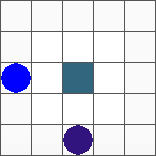
\includegraphics[scale=0.8]{figs/casestudy2.png}
		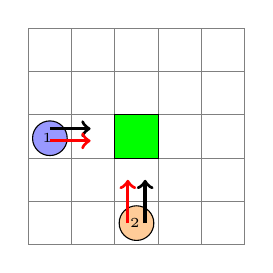
\begin{tikzpicture}[scale=1.1]
		\draw[step=0.5cm,color=gray] (-1.5,-1.5) grid (1,1);
		%\filldraw[fill=blue,draw=black] (-1.28,-0.27) circle (0.2cm);
		\filldraw[fill=green,draw=black] (0,0) rectangle (-0.5,-0.5);
		%\filldraw[fill=red,draw=black] (-0.5,0) rectangle (-1,-0.5);
		%\filldraw[fill=red,draw=black] (0,0) rectangle (0.5,-0.5);
		\filldraw[fill=blue!40!white,draw=black] (-1.25,-0.27) circle (0.2cm);
		\draw[very thick,->,black] (-1.25,-0.16) -- (-0.78,-0.16);
		\draw[very thick,->,red] (-1.25,-0.3) -- (-0.78,-0.3);
		\filldraw[fill=orange!40!white,draw=black] (-0.25,-1.25) circle (0.2cm);
		\draw[very thick,->,black] (-0.15,-1.25) -- (-0.15,-0.75);
		\draw[very thick,->,red] (-0.35,-1.25) -- (-0.35,-0.75);
		\node at (-1.28,-0.27) {\tiny{1}};
		\node at (-0.27,-1.25) {\tiny{2}};
		\end{tikzpicture}
	}
	%\hfill
	\subfloat[$t_2$ \label{fig:t2}]{
		%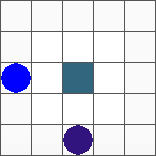
\includegraphics[scale=0.8]{figs/casestudy2.png}
		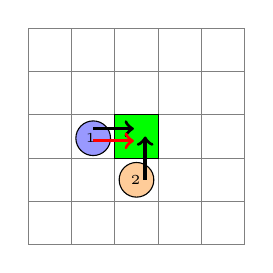
\begin{tikzpicture}[scale=1.1]
		\draw[step=0.5cm,color=gray] (-1.5,-1.5) grid (1,1);
		%\filldraw[fill=blue,draw=black] (-1.28,-0.27) circle (0.2cm);
		\filldraw[fill=green,draw=black] (0,0) rectangle (-0.5,-0.5);
		%\filldraw[fill=red,draw=black] (-0.5,0) rectangle (-1,-0.5);
		%\filldraw[fill=red,draw=black] (0,0) rectangle (0.5,-0.5);
		\filldraw[fill=blue!40!white,draw=black] (-0.75,-0.27) circle (0.2cm);
		\draw[very thick,->,black] (-0.75,-0.16) -- (-0.28,-0.16);
		\draw[very thick,->,red] (-0.75,-0.3) -- (-0.28,-0.3);
		\filldraw[fill=orange!40!white,draw=black] (-0.25,-0.75) circle (0.2cm);
		\draw[very thick,->,black] (-0.15,-0.75) -- (-0.15,-0.25);
		%\draw[very thick,->,red] (-0.35,-0.75) -- (-0.35,-0.25);
		\node at (-0.78,-0.27) {\tiny{1}};
		\node at (-0.26,-0.75) {\tiny{2}};
		\end{tikzpicture}
	}\subfloat[$t_3$ \label{fig:t3}]{
		%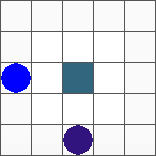
\includegraphics[scale=0.8]{figs/casestudy2.png}
		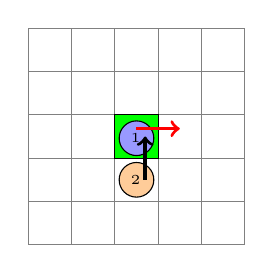
\begin{tikzpicture}[scale=1.1]
		\draw[step=0.5cm,color=gray] (-1.5,-1.5) grid (1,1);
		%\filldraw[fill=blue,draw=black] (-1.28,-0.27) circle (0.2cm);
		\filldraw[fill=green,draw=black] (0,0) rectangle (-0.5,-0.5);
		%\filldraw[fill=red,draw=black] (-0.5,0) rectangle (-1,-0.5);
		%\filldraw[fill=red,draw=black] (0,0) rectangle (0.5,-0.5);
		\filldraw[fill=blue!40!white,draw=black] (-0.25,-0.27) circle (0.2cm);
		%\draw[very thick,->,black] (-0.25,-0.16) -- (-0.78,-0.16);
		\draw[very thick,->,red] (-0.25,-0.16) -- (0.25,-0.16);
		\filldraw[fill=orange!40!white,draw=black] (-0.25,-0.75) circle (0.2cm);
		\draw[very thick,->,black] (-0.15,-0.75) -- (-0.15,-0.25);
		%\draw[very thick,->,red] (-0.35,-1.25) -- (-0.35,-0.75);
		\node at (-0.26,-0.27) {\tiny{1}};
		\node at (-0.26,-0.75) {\tiny{2}};
		\end{tikzpicture}
	}
	
	\subfloat[$t_4$\label{fig:t4}]{
	%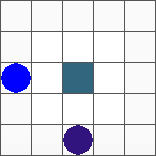
\includegraphics[scale=0.8]{figs/casestudy2.png}
	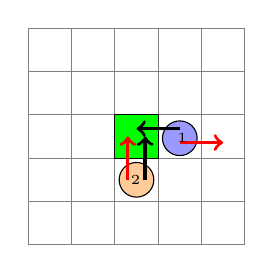
\begin{tikzpicture}[scale=1.1]
	\draw[step=0.5cm,color=gray] (-1.5,-1.5) grid (1,1);
	%\filldraw[fill=blue,draw=black] (-1.28,-0.27) circle (0.2cm);
	\filldraw[fill=green,draw=black] (0,0) rectangle (-0.5,-0.5);
	%\filldraw[fill=red,draw=black] (-0.5,0) rectangle (-1,-0.5);
	%\filldraw[fill=red,draw=black] (0,0) rectangle (0.5,-0.5);
	\filldraw[fill=blue!40!white,draw=black] (0.25,-0.27) circle (0.2cm);
	\draw[very thick,->,black] (0.25,-0.16) -- (-0.25,-0.16);
	\draw[very thick,->,red] (0.25,-0.32) -- (0.75,-0.32);
	\filldraw[fill=orange!40!white,draw=black] (-0.25,-0.75) circle (0.2cm);
	\draw[very thick,->,black] (-0.15,-0.75) -- (-0.15,-0.25);
	\draw[very thick,->,red] (-0.35,-0.75) -- (-0.35,-0.25);
	\node at (0.28,-0.27) {\tiny{1}};
	\node at (-0.26,-0.75) {\tiny{2}};
	\end{tikzpicture}
	}
	\subfloat[$t_5$\label{fig:t5}]{
	%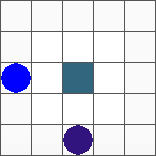
\includegraphics[scale=0.8]{figs/casestudy2.png}
	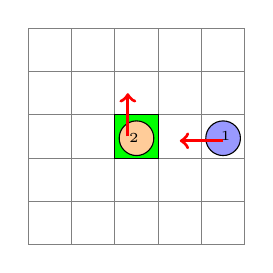
\begin{tikzpicture}[scale=1.1]
	\draw[step=0.5cm,color=gray] (-1.5,-1.5) grid (1,1);
	%\filldraw[fill=blue,draw=black] (-1.28,-0.27) circle (0.2cm);
	\filldraw[fill=green,draw=black] (0,0) rectangle (-0.5,-0.5);
	%\filldraw[fill=red,draw=black] (-0.5,0) rectangle (-1,-0.5);
	%\filldraw[fill=red,draw=black] (0,0) rectangle (0.5,-0.5);
	\filldraw[fill=blue!40!white,draw=black] (0.75,-0.27) circle (0.2cm);
	%\draw[very thick,->,black] (-1.25,-0.16) -- (-0.78,-0.16);
	\draw[very thick,->,red] (0.75,-0.3) -- (0.25,-0.3);
	\filldraw[fill=orange!40!white,draw=black] (-0.25,-0.27) circle (0.2cm);
	%\draw[very thick,->,black] (-0.15,-1.25) -- (-0.15,-0.75);
	\draw[very thick,->,red] (-0.35,-0.25) -- (-0.35,0.25);
	\node at (-0.28,-0.27) {\tiny{2}};
	\node at (0.78,-0.25) {\tiny{1}};
	\end{tikzpicture}
	}\subfloat[$t_6$ \label{fig:t6}]{
	%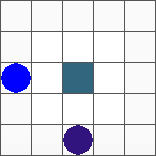
\includegraphics[scale=0.8]{figs/casestudy2.png}
	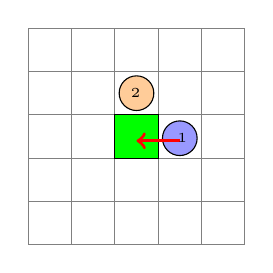
\begin{tikzpicture}[scale=1.1]
	\draw[step=0.5cm,color=gray] (-1.5,-1.5) grid (1,1);
	%\filldraw[fill=blue,draw=black] (-1.28,-0.27) circle (0.2cm);
	\filldraw[fill=green,draw=black] (0,0) rectangle (-0.5,-0.5);
	%\filldraw[fill=red,draw=black] (-0.5,0) rectangle (-1,-0.5);
	%\filldraw[fill=red,draw=black] (0,0) rectangle (0.5,-0.5);
	\filldraw[fill=blue!40!white,draw=black] (0.25,-0.27) circle (0.2cm);
	%\draw[very thick,->,black] (-1.25,-0.16) -- (-0.78,-0.16);
	\draw[very thick,->,red] (0.25,-0.3) -- (-0.25,-0.3);
	\filldraw[fill=orange!40!white,draw=black] (-0.25,0.25) circle (0.2cm);
	%\draw[very thick,->,black] (-0.15,-1.25) -- (-0.15,-0.75);
	%\draw[very thick,->,red] (-0.35,-1.25) -- (-0.35,-0.75);
	\node at (-0.26,+0.25) {\tiny{2}};
	\node at (0.28,-0.27) {\tiny{1}};
	\end{tikzpicture}
	}
	
	
	\caption[Gridworld simulaiton of multi-agent shielding interference]{Green cell is the charging station. Black arrows correspond to intended actions (outputs from the system) and red arrows correspond to shield outputs. The absence of an arrow indicates that the action chosen was to stay at the same cell. In \ref{fig:t1}, no interference is needed. In the next time step in \ref{fig:t2}, the shield interferes with agent 2 to prevent collision in the charging area. In \ref{fig:t3}, the shield forces agent 1 out of charging area, and agent 2 to wait one time-step as agent 2 is not allowed to enter immediately after agent 1 leaves. In the following 3 figures, Agent 2 is allowed to charge while agent 1 is not allowed back and then Agent 2 is forced out to prepare for agent 1 to charge before finally Agent 1 is forced into the charging station. }
	\label{fig:casestudies}
\end{figure}


\subsection{UAV mission planning}\label{sec:results_casestudy}
We synthesized shields for 3 unmanned aerial vehicles (UAVs) simulated using ROS/Gazebo for the case study outlined in Section \ref{sec:casestudy}. As shown in Figure \ref{fig:warehouse}, the environment consists of 2 rows of shelves. We assume there are 12 discrete package pick up points in each row of shelves along with the drop off location and charging station. The input of each UAV controller is its location in $(x,y,z)$. The possible outputs of each UAV consist of 17 trajectories precomputed using a minimum-snap trajectory generator that moves the UAV from one discrete state to another.
We consider a safety specification $\spec_{dist}$ which captures the requirement that the controllers should not choose trajectories that bring them within distance less than a given threshold $r$. The output of each UAV is chosen from the set $T = \{1,2,\ldots,17\}$ where each integer corresponds to a particular trajectory choice. Let the function $dist: T \times T \to \nats$  map each pair of trajectories $traj_i,traj_j \in T$ to the closest distance between them. 
We define the safety specification as
  \begin{align}
  \spec_{dist}&= \LTLglobally \LTLand_{i\neq j}\Big(dist(traj_i,traj_j) \geq r\Big).
  \end{align}
 Additionally, we specify $\spec_{shelf}$ which states that no more than one UAV can move into the row of shelves at the same time. Lastly, like \ref{exp:gridworld}, only one UAV can be at the charging station or drop-off point at any given time and UAVs cannot be allowed to run out of power when not in a charging station. 

We assign a higher cost to the interference with the orange UAV compared to the other two. Intuitively, this will force the shield, where possible, to avoid interfering with the orange UAV. We synthesize the shield for two different values of $b$ and the synthesis times are reported in Table~\ref{tab:exp1} under case (2). A video of the simulation can be seen in \url{https://bit.ly/2OSRhxJ}.

